\documentclass{article}
%XXXXXXXXXXXXXXXXXXXXXXXXXXXXXXXXXXXXXXXXXXXXXXXXXXXXXXXXXXXXXXXXXXXXXXXXXXXXXXXXXXXXXXXXXXXXXXXXXXXXXXXXXXXXXXXX
% Standard packages
\usepackage{amsmath}        % Extra math definitions
\usepackage{setspace}       % 1.5 spacing
\usepackage{latexsym}
\usepackage{amsfonts}
\usepackage{amssymb}
\usepackage{color}
%\usepackage{natbib}
%\usepackage{nicefrac}
\usepackage{hyperref}
\usepackage{theorem}
\usepackage{graphicx}
%XXXXXXXXXXXXXXXXXXXXXXXXXXXXXXXXXXXXXXXXXXXXXXXXXXXXXXXXXXXXXXXXXXXXXXXXXXXXXXXXXXXXXXXXXXXXXXXXXXXXXXXXXXXXXXXXX
% Custom packages
\allowdisplaybreaks
%\usepackage[all]{datestamp}   % Datestamp on first page of each chapter
%\usepackage{fancyhdr}
%\input{defs.sty}          % Commands
\input{commands.txt}      % Commands
\def\Red{\special{color cmyk 0 1. 1. 0}} % PANTONE RED
%\newcommand{\var}{\operatorname{var}}
%\newcommand{\cov}{\operatorname{cov}}
\def\Black{\special{color cmyk 0 0 0 1.}} % PANTONE PROCESS-BLACK
\def\Green{\special{color cmyk 0.64 0 0.95 0.3}} % PANTONE 582
\def\Blue{\special{color cmyk 1. 1. 0 0}} % PANTONE BLUE-072
%\usepackage{bib}
\addtolength{\textwidth}{4cm} \addtolength{\oddsidemargin}{-2cm}
%   XXXXXXXXXXXXXXXXXXXXXXXXXXXXXXXXXXXXXXXXXXXXXXXXXXXXXXXXXXXXXXXXXXXXXXXXXXXXXXXXXXXXXXXXXXXXXXXXXXXXXXXXXXXXXXXX
%===== page layout
\title{Sketch of proof of important calculus rule for quadratic covariations \\ QF\footnote{If you have comments/questions please send an e-mail
to \textcolor{blue}{\href{mailto:r.vdnakker@uvt.nl}{r.vdnakker@uvt.nl}} } }
\date{ }

%========= Document start =====================================================================
\begin {document}
\maketitle
%===== Title page
\noindent
\textbf{Calculus rule} \\
If $X$ is a solution to the SDE $\rd X_t=\mu_t \rd t + \sigma_t \rd W_t$, with $W_1\distr \rN(0,1)$ 
and $Y$ is another process with continuous sample paths then we have $\rd [X,Y]_t=\sigma_t \rd [W,Y]_t$. In particular,
$\rd [X,X]_t=\sigma_t^2 \rd [W,W]_t=\sigma_t^2 \rd t$.
\\ \\
\textbf{Sketch of proof} \\
Fix $T>0$. \\
\underline{Step 1} \\
Introduce the processes $m$ and $Z$ by $m_t=\int_0^t \mu_u \rd u$ and $Z_t=\int_0^t \sigma_u \rd W_u$. Since $m$ is of Bounded variation we have
$[X,Y]_T=[m+Z,Y]_T=[Z,Y]_T$. \\
\underline{Step 2} \\
First we consider simple processes $\sigma_t$. This means that there exists $M\in\SN$ and $0=s_0<\dots<s_M=T$
such that $\sigma_t=\sum_{j=1}^M \sigma^j 1_{[s_{j-1},s_j)}(t)+\sigma^M 1_{\{T\}}(t)$, with $\sigma^j$ $\calF_{s_{j-1}}$-measurable.
Next we consider partitions $0=s_0=t_0<\dots<t_m=s_1<\dots<t_{2m}=s_2<\dots<t_{Mm}=s_M=T$, $n=Mm$. See Figure~\ref{fig} for an illustration.
\begin{figure}
\begin{center}
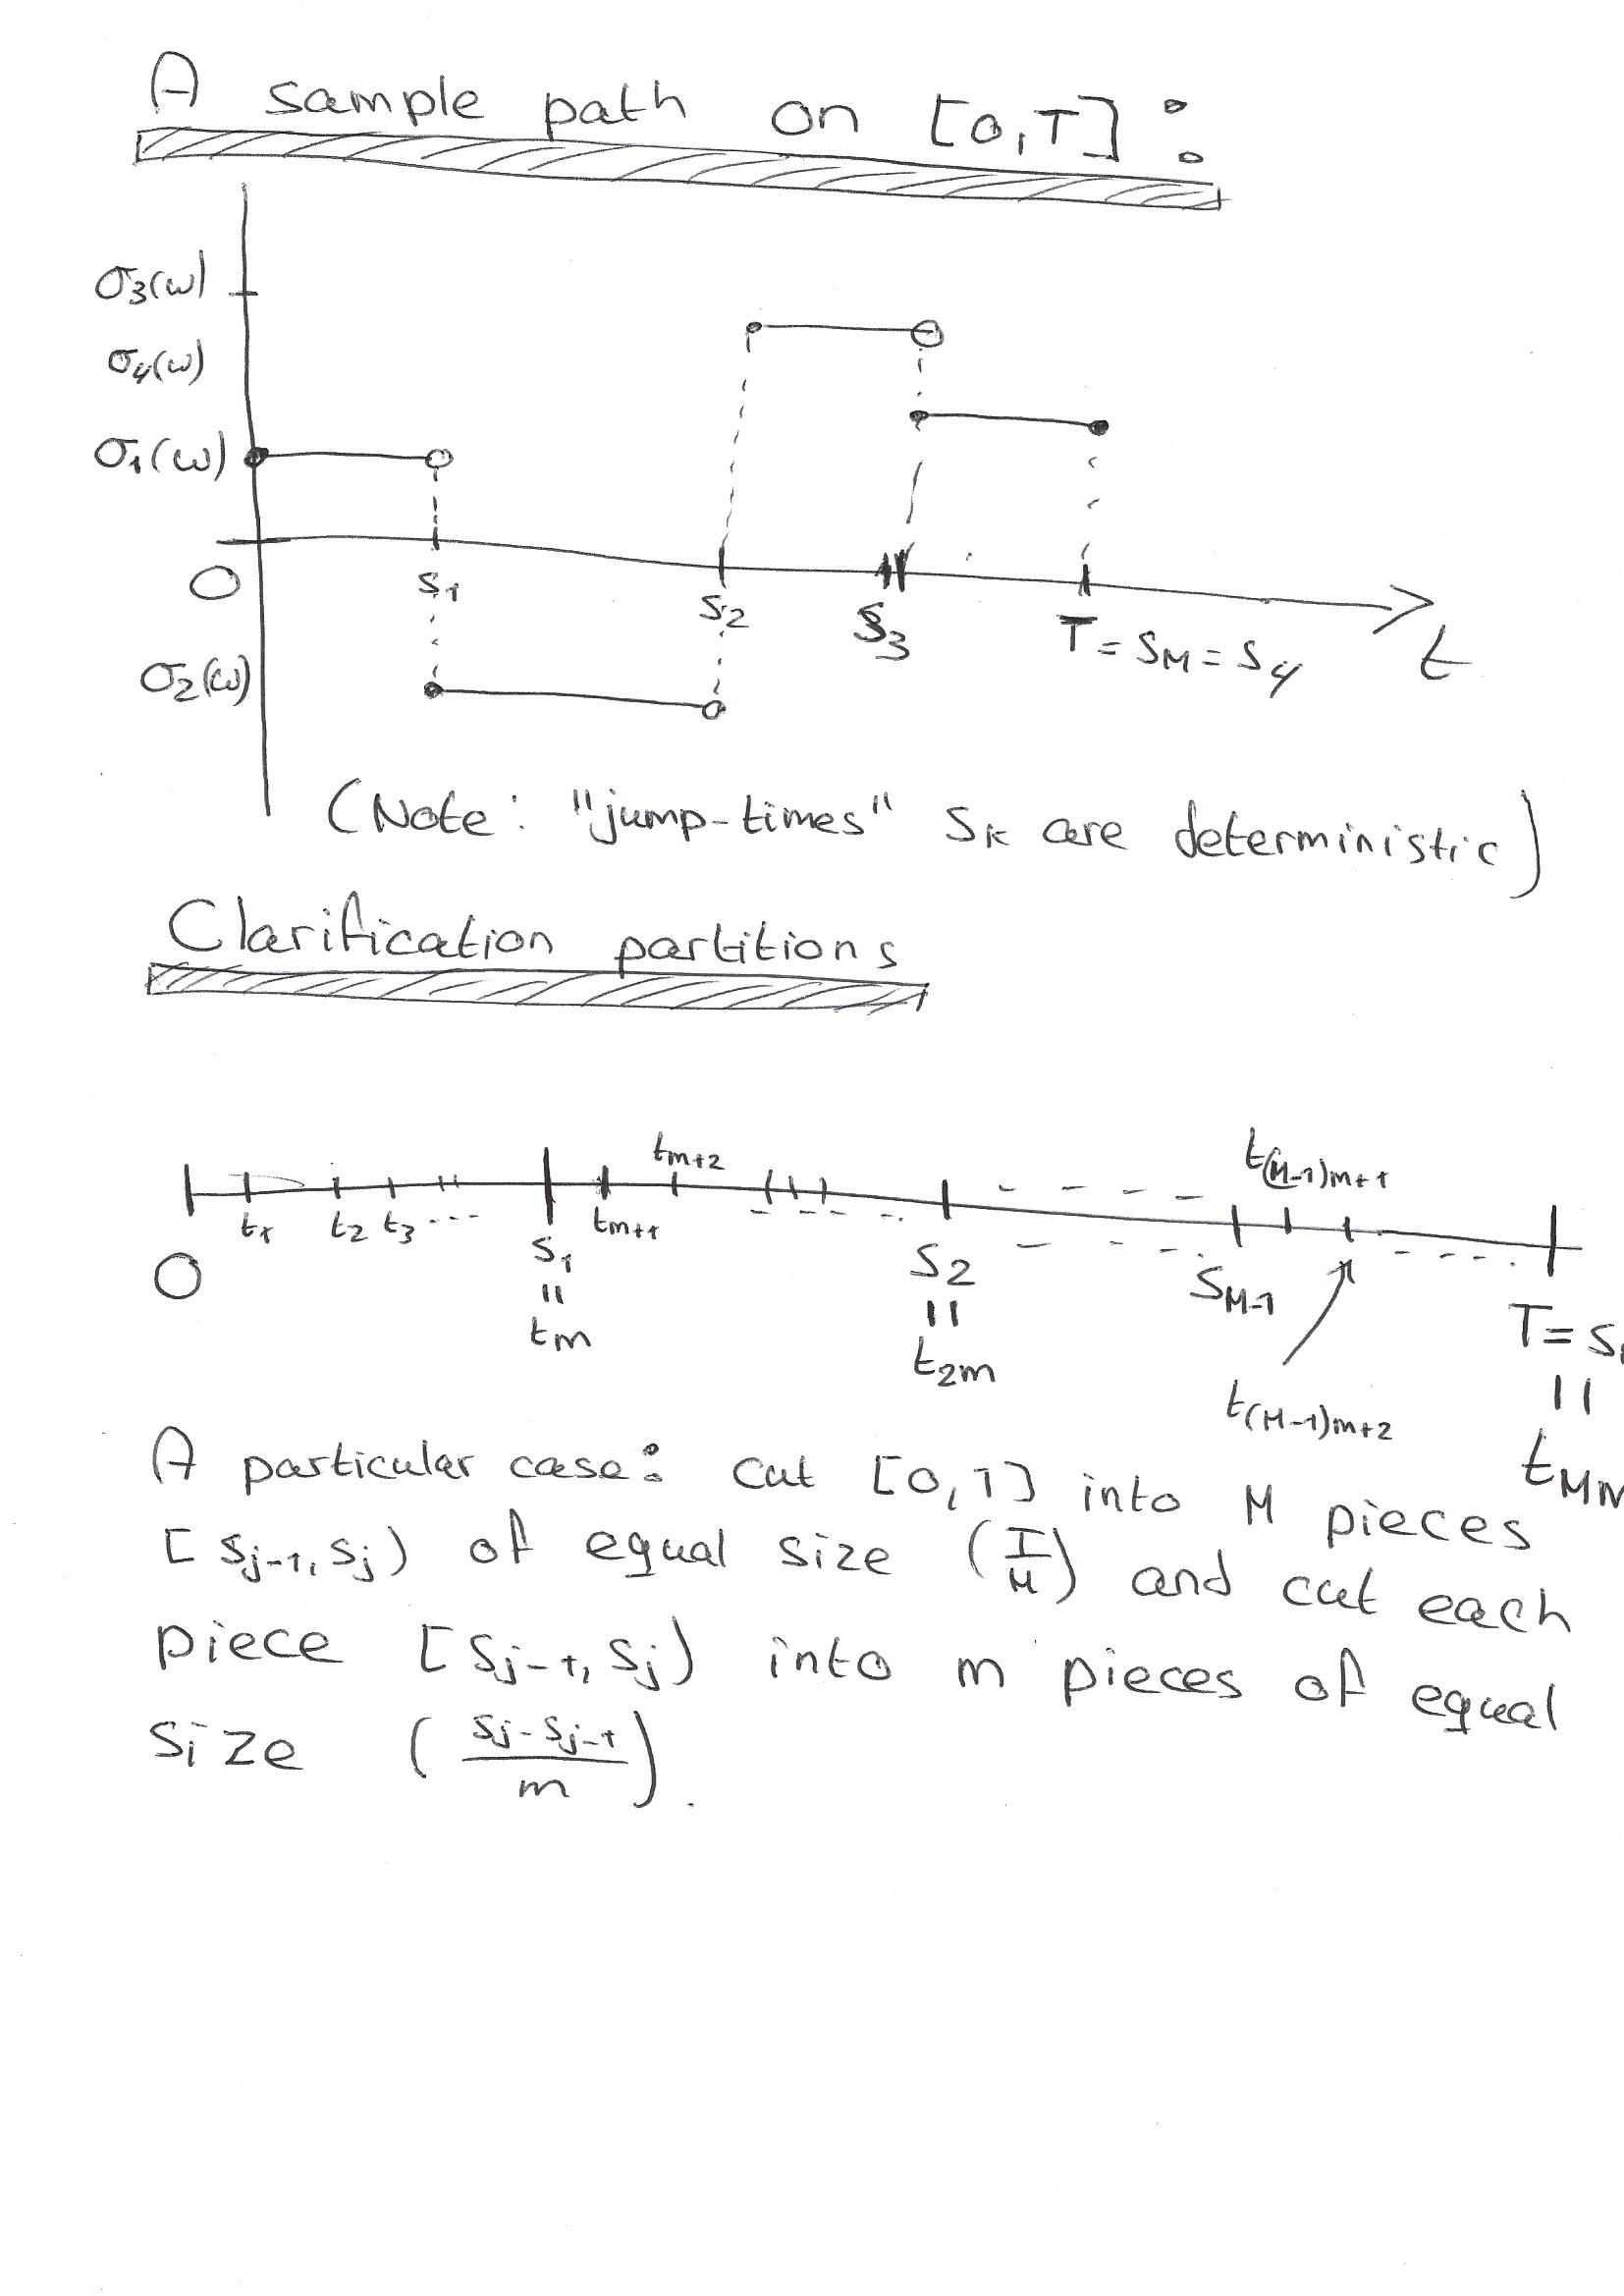
\includegraphics[height=0.85\textwidth]{Scan.jpg}
\caption{Illustration of `simple processes'  and the partitions.}\label{fig}
\end{center}
\end{figure}
Now notice that
\begin{align*}
[Z,Y]_T&=\operatorname{plim}_{m\to\infty}
\sum_{k=1}^n (Z_{t_k}-Z_{t_{k-1}})(Y_{t_k}-Y_{t_{k-1}})
=\operatorname{plim}_{m\to\infty}\sum_{j=1}^{M} \sum_{k=(j-1)m+1}^{jm}   (Z_{t_k}-Z_{t_{k-1}})(Y_{t_k}-Y_{t_{k-1}})
\\
&=\operatorname{plim}_{m\to\infty}
\sum_{j=1}^M
\sum_{k=(j-1)m+1}^{jm} \sigma^j (W_{t_k}-W_{t_{k-1}})(Y_{t_k}-Y_{t_{k-1}})
\\
&=
\sum_{j=1}^M \sigma^j \operatorname{plim}_{m\to\infty} \sum_{k=(j-1)m+1}^{jm}  (W_{t_k}-W_{t_{k-1}})(Y_{t_k}-Y_{t_{k-1}})
\\
&=
\sum_{j=1}^M \sigma^j \left( [W,Y]_{s_j} -[W,Y]_{s_{j-1}}\right)=\int_0^T \sigma_u \rd [W,Y]_u.
\end{align*}
So the theorem holds for simple processes.
\\
\underline{Step 3} \\
Next we consider general $\sigma_t$. There exists a sequence of simple processes $\sigma^{(n)}$ with $\sigma^{(n)}_t(\omega)\to \sigma_t(\omega)$ for almost all $(t,\omega)$ (this is a standard construction technique from measure theory).
Now define processes $Z^{(n)}$ by $Z^{(n)}_t=\int_0^t\sigma^{(n)}_u \rd W_u$.
Now we have
\begin{align*}
[X,Y]_T&=[Z,Y]_T=[ \operatorname{plim}_{n\to\infty} Z^{(n)},Y]_T\stackrel{?}{=}\operatorname{plim}_{n\to\infty}[ Z^{(n)},Y]_T \\
&=\operatorname{plim}_{n\to\infty} \int_0^T \sigma^{(n)}_u \rd [W,Y]_u
\stackrel{?}{=}\int_0^T\operatorname{plim}_{n\to\infty} \sigma^{(n)}_u \rd [W,Y]_u= \int_0^T \sigma_u \rd [W,Y]_u,
\end{align*}
which concludes the proof.
Notice that we interchanged the order of operations (limits and integrals) several times. To justify this conditions have to be satisfied, which we do not discuss in the sketch of the proof (and in the formulation of the result).
\end{document}
